\documentclass[tikz,border=4pt]{standalone}
\usepackage{amsmath}
\usepackage{xcolor}
\usepackage{tikz}
\usepackage{pgfplots}
\pgfplotsset{compat=1.18}

\definecolor{caraprimary}{RGB}{30,60,120}
\definecolor{caraaccent}{RGB}{200,80,60}

\begin{document}
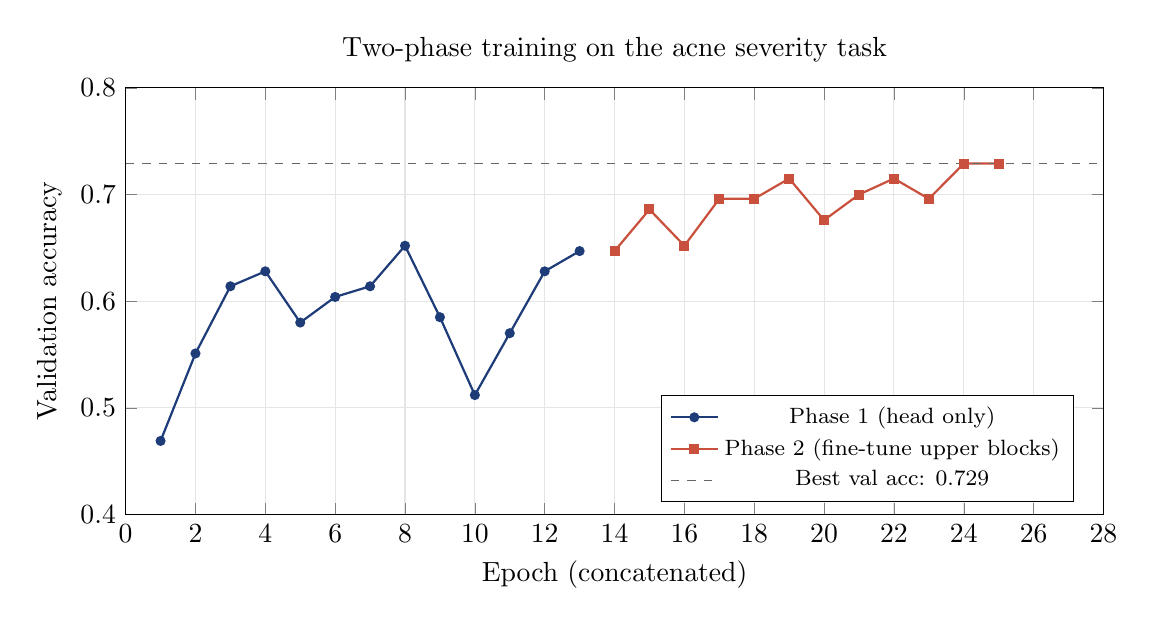
\begin{tikzpicture}
\begin{axis}[
    width=14cm, height=7cm,
    xlabel={Epoch (concatenated)}, ylabel={Validation accuracy},
    ymin=0.4, ymax=0.8,
    xmin=0, xmax=28,
    grid=both, grid style={gray!20},
    legend pos=south east,
    legend style={font=\footnotesize},
    title={Two-phase training on the acne severity task}]
\addplot[thick, color=caraprimary, mark=*, mark size=1.4pt] coordinates {
    (1,0.469) (2,0.551) (3,0.614) (4,0.628) (5,0.580)
    (6,0.604) (7,0.614) (8,0.652) (9,0.585) (10,0.512)
    (11,0.570) (12,0.628) (13,0.647)
};
\addlegendentry{Phase 1 (head only)}
\addplot[thick, color=caraaccent, mark=square*, mark size=1.4pt] coordinates {
    (14,0.647) (15,0.686) (16,0.652) (17,0.696) (18,0.696)
    (19,0.715) (20,0.676) (21,0.700) (22,0.715) (23,0.696)
    (24,0.729) (25,0.729)
};
\addlegendentry{Phase 2 (fine-tune upper blocks)}
\addplot[dashed, color=black!60] coordinates {(0,0.729) (28,0.729)};
\addlegendentry{Best val acc: 0.729}
\end{axis}
\end{tikzpicture}
\end{document}
